\documentclass[11pt]{article}
\usepackage{fullpage}
\usepackage{amsmath,amssymb,amsthm}
\usepackage{array,booktabs,longtable}
\usepackage{tikz}
\usepackage{float}
\usepackage{placeins}
\usepackage[obeyspaces,spaces]{url}
\usepackage[colorlinks=true,linkcolor=blue,citecolor=blue,urlcolor=blue]{hyperref}
% The author's macros.
%
% some calligraphy
%
\newcommand\cA{{\mathcal A}}
\newcommand\cB{{\mathcal B}}
\newcommand\cC{{\mathcal C}}
\newcommand\cD{{\mathcal D}}
\newcommand\cE{{\mathcal E}}
\newcommand\cF{{\mathcal F}}
\newcommand\cG{{\mathcal G}}
\newcommand\cH{{\mathcal H}}
\newcommand\cI{{\mathcal I}}
\newcommand\cJ{{\mathcal J}}
\newcommand\cK{{\mathcal K}}
\newcommand\cL{{\mathcal L}}
\newcommand\cM{{\mathcal M}}
\newcommand\cN{{\mathcal N}}
\newcommand\cP{{\mathcal P}}
\newcommand\cQ{{\mathcal Q}}
\newcommand\cR{{\mathcal R}}
\newcommand\cS{{\mathcal S}}
\newcommand\cT{{\mathcal T}}
\newcommand\cU{{\mathcal U}}
\newcommand\cV{{\mathcal V}}

%
% fields and rings (and a semigroup)
%
\newcommand\cx{{\mathbb C}}% complexes
\newcommand\fld{{\mathbb F}}
\newcommand\flde{{\mathbb E}}
\newcommand\ints{{\mathbb Z}}
\newcommand\nn{{\mathbb N}}%non-negative integers
\newcommand\re{{\mathbb R}}%reals
\newcommand\rats{{\mathbb Q}}

\newcommand\Zu{{\mathbf u}}
\newcommand\Zv{{\mathbf v}}
\newcommand\Zw{{\mathbf w}}
\newcommand\Zy{{\mathbf y}}
\newcommand\Zz{{\mathbf z}}
\newcommand\Zx{{\mathbf x}}
\newcommand\Zj{{\mathbf j}}


%
% the really useful stuff
%
%\newcommand\opk[1]{\mathop{\hbox{\rm #1}}\nolimits} %% old version
\newcommand\opk[1]{\mathop{\mathrm{#1}}\nolimits}
\newcommand\comp[1]{{\mkern2mu\overline{\mkern-2mu#1}}}
\newcommand\diff{\mathbin{\mkern-1.5mu\setminus\mkern-1.5mu}}% for \setminus
\newcommand\gbin[2]{\genfrac{[}{]}{0pt}{}{#1}{#2}}
\newcommand\inv{^{-1}}
\newcommand\res{\mathbin{\mkern-2.0mu\restriction\mkern-2.0mu}}% ch2
\newcommand\sbs{\subseteq}
\newcommand\sps{\supseteq}
\newcommand\seq[3]{#1_{#2},\ldots,#1_{#3}}
\newcommand\supp{\opk{supp}}
\newcommand\im{\opk{im}}
\newcommand\row{\opk{row}}
\newcommand\pmat[1]{\begin{pmatrix} #1 \end{pmatrix}}
\newcommand\cprod{\mathbin{\square}}
%
% matrix theory
%
\newcommand\ip[2]{\langle#1,#2\rangle}
\newcommand\one{{\bf1}}
\newcommand\rk{\opk{rk}}
\newcommand\tr{\opk{tr}}
\newcommand\col{\opk{col}}
\newcommand\mat[3]{\mathrm{Mat}_{#1\times #2}(#3)}

%
% some group theory
%
\newcommand\aut[1]{{\rm Aut}(#1)}
\newcommand\fx[1]{{\rm fix}(#1)}% ch2
\newcommand\grp[1]{\langle #1\rangle}
\newcommand\nrml{\vartriangleleft}
\newcommand\nrmleq{\trianglelefteq}
\newcommand\alt[1]{\opk{Alt}(#1)}
\DeclareMathOperator{\Sym}{Sym}
% End of the author's macros.
\newtheorem{theorem}{Theorem}[section]
\newtheorem{lemma}[theorem]{Lemma}
\newtheorem{proposition}[theorem]{Proposition}
\newtheorem{corollary}[theorem]{Corollary}
\theoremstyle{definition}
\newtheorem{definition}[theorem]{Definition}
\newtheorem{remark}[theorem]{Remark}
\DeclareRobustCommand{\ml}[1]{\ifmmode\text{\normalfont\small\ttfamily\detokenize{#1}}\else{\normalfont\small\nolinkurl{#1}}\fi}
\newcommand{\typ}[1]{\mathrm{#1}}
\newcommand{\lmin}{\lambda_{\min}}
\newcommand\Ze{{\mathbf e}}
\newcommand\Zs{{\mathbf s}}
\newcommand\Zp{{\mathbf p}}
\renewcommand{\labelenumi}{(\theenumi)}
\renewcommand{\floatpagefraction}{0.7}
\emergencystretch=2em
\title{A database of exceptional graphs\\ with least eigenvalue $\ge-2$}
\author{Krystal Guo\\
\normalsize Korteweg-de Vries Institute for Mathematics, University of Amsterdam\\
\normalsize\texttt{k.guo@uva.nl}}
\date{2 November 2026}

\begin{document}
\raggedbottom
\maketitle
\begin{abstract}
There are exactly $54\,732\,619$ exceptional graphs up to isomorphism, that is, connected graphs
with least eigenvalue at least $-2$ that are not generalized line graphs. There are $54\,732\,046$ with
least eigenvalue $-2$, on $7$ to $36$ vertices, and $573$ with least eigenvalue strictly greater than
$-2$, on $6$, $7$ and $8$ vertices. By theorems of Cameron, Goethals, Seidel and Shult, an
exceptional graph is represented in the root system $\typ E_8$ and has at most $36$ vertices, so
there are finitely many; Cvetkovi\'c wrote in 2004 that their number is very big but not known.
We prove that a connected graph with least eigenvalue at least $-2$ is represented in $\typ E_8$
if and only if the rank of $2I+A$ is at most $8$, with $A$ the adjacency matrix, and that it is
exceptional if and only if the pair formed by this rank and the determinant of the lattice
spanned by its representation is $(6,3)$, $(7,2)$ or $(8,1)$. We show how to find, by exact
tests on integer matrices, every way of adding a vertex to a connected graph represented in
$\typ E_8$ resulting in a connected graph that is also represented in $\typ E_8$.
We then generate the $54\,752\,217$ connected graphs represented in $\typ E_8$, one vertex at a time,
and thus produce a database of all exceptional graphs, up to isomorphism, which we make available.
We obtained these results in the course of
autoformalizing the paper of Cameron, Goethals, Seidel and Shult in the proof assistant Lean.

\end{abstract}

\section{Introduction}\label{sec:intro}

We consider graphs with least eigenvalue at least $-2$, where by eigenvalues of a graph we mean
those of its adjacency matrix. Line graphs have least eigenvalue at least $-2$, and so do the
cocktail party graphs $CP(m)$ ($K_{2m}$ minus a perfect matching). We recall that the
\textsl{line graph} $L(Y)$ of a graph $Y$ has the edges of $Y$ as its vertices, two of them
adjacent when they are incident with a common vertex of $Y$. For a graph $Y$ on the vertices
$1,\dots,m$ and integers $a_1,\dots,a_m\ge0$, the \textsl{generalized line graph}
$L(Y;a_1,\dots,a_m)$, of~\cite[\S4]{CGSS} and~\cite[\S1.1]{CRS04}, is obtained from $L(Y)$ by
adding disjoint cocktail party graphs $CP(a_1),\dots,CP(a_m)$, with every vertex of $CP(a_i)$
adjacent to every vertex of $L(Y)$ that, as an edge of $Y$, contains the vertex $i$. A graph $X$
is \textsl{exceptional} if it is connected, its least eigenvalue $\lmin(X)$ is at least $-2$, and
$X$ is not a generalized line graph~\cite[\S1.1]{CRS04}. The classical result of Cameron,
Goethals, Seidel and Shult~\cite{CGSS} tells us that a connected graph with least eigenvalue at
least $-2$ is either a generalized line graph or an exceptional graph, of which there are a
finite number.

More specifically, they showed this by representing the exceptional graphs in the root system
$\typ E_8$. A \textsl{representation} of a graph $X$ is a family of vectors $\Zx_u$
($u\in V(X)$) in a real inner product space with $\ip{\Zx_u}{\Zx_u}=2$ and
$\ip{\Zx_u}{\Zx_w}=A(u,w)$ for $u\ne w$, where $A=A(X)$ is the adjacency matrix of $X$. It is a
representation in $\typ E_8$ if every $\Zx_u$ is a root of $\typ E_8$, and we say that $X$ is
\textsl{represented in} $\typ E_8$ if it has such a representation; we will recall the root
systems in Section~\ref{sec:lattices}. By~\cite[Theorem~4.10]{CGSS}, a connected graph with least
eigenvalue at least $-2$ is a generalized line graph or is represented in $\typ E_8$; the theorem
is stated for least eigenvalue $-2$ and leaves connectedness implicit, but its proof uses only
that the graph is connected and that $\lmin\ge-2$. Thus every
exceptional graph is represented in $\typ E_8$ and, by~\cite[Theorem~4.3]{CGSS}, has at most
$36$ vertices. The only fact about generalized line graphs that our proofs use
is~\cite[Theorem~4.2]{CGSS}: a graph is a generalized line graph if and only if it is
represented in $\typ D_\ell$ for some $\ell$ (Section~\ref{sec:lattices}).

The exceptional graphs with $\lmin>-2$ are classical: there are $573$ of them, $20$ on $6$
vertices, $110$ on $7$ and $443$ on $8$~\cite[\S2.3 and Table~A2]{CRS04}, \cite{DC79}. The
maximal exceptional graphs were found by Cvetkovi\'c, Lepovi\'c, Rowlinson and Simi\'c with the
star complement technique: there are $473$ of them, on $22$ to $36$
vertices~\cite{CLRS02}, \cite[Chapter~6]{CRS04}. In 2004, Cvetkovi\'c wrote~\cite{Cve04}:
\begin{quote}
The set $E$ of exceptional graphs is finite. The number of exceptional graphs is very big but
not known. The set $E$ can be partially ordered by the induced subgraph relation. In this order
$E$ has 20 minimal elements and 473 maximal ones.
\end{quote}

In this note we determine the very big number.

\begin{theorem}\label{thm:count}
There are exactly $54\,732\,619$ exceptional graphs up to isomorphism: $54\,732\,046$ with
least eigenvalue $-2$, on $7$ to $36$ vertices, and $573$ with least eigenvalue greater than
$-2$, on $6$, $7$ and $8$ vertices. For each $n$, the number of exceptional graphs on $n$
vertices is given in Table~\ref{tab:counts}.
\end{theorem}

We also produce a database of all exceptional graphs (one for each isomorphism class), which we
make available, with our code and the formalization in Lean, at
\url{https://github.com/kguo-sagecode/least-eig-minus-2}, archived on Zenodo as
\url{https://doi.org/10.5281/zenodo.23925794}.

The proof of Theorem~\ref{thm:count} is a computation, but not a direct computation. The root
system $\typ E_8$ has $240$ roots, which lie on $120$ lines through the origin of
$\re^8$~\cite[Lemma~3.4]{CGSS}, and the inner product of two roots on different lines is $0$,
$1$ or $-1$. In a representation, distinct vertices have distinct roots, with inner product $0$
or $1$. Thus a representation in $\typ E_8$ of a graph on $n$ vertices is the same thing as a
set of $n$ lines of $\typ E_8$ with a root chosen on each line so that no two chosen roots have
inner product $-1$, and the graph is recovered from it: two vertices are adjacent when their
roots have inner product $1$. In principle, then, the exceptional graphs could be found by
running through the sets of at most $36$ of the $120$ lines, with a root chosen on each line. But
there are more than $4\cdot10^{41}$ such choices, and even the group of symmetries of
$\typ E_8$, which has order $696\,729\,600$~\cite[Chapter~4]{CS99}, reduces them to no fewer than
$6\cdot10^{32}$ orbits. Since it is also computationally infeasible to go through the more than
$10^{148}$ graphs on $36$ vertices up to isomorphism, it was necessary to establish the lemmas
of Sections~\ref{sec:lattices} and~\ref{sec:growth}, which make our enumeration feasible in four
ways.

First, two integers decide whether a connected graph $X$ with $\lmin(X)\ge-2$ is represented
in $\typ E_8$ and whether it is exceptional. With $M(X)=2I+A(X)$ and $\Lambda(X)$ the lattice
spanned by a representation of $X$, the graph $X$ is represented in $\typ E_8$ if and only if
$\rk M(X)\le8$, and it is exceptional if and only if the pair $(\rk M(X),\det\Lambda(X))$ is
$(6,3)$, $(7,2)$ or $(8,1)$ (Proposition~\ref{prop:types}). Both integers
$(\rk M(X),\det\Lambda(X))$ are computed exactly. Note that we do not need to compute any
eigenvalues, since $\lmin(X)=-2$ if and only if $\rk M(X)<n$.

Second, a connected graph on at least two vertices represented in $\typ E_8$ has a vertex whose
deletion leaves a connected graph represented in $\typ E_8$ (Lemma~\ref{lem:noncut}). Thus the
connected graphs represented in $\typ E_8$ can be generated one vertex at a time, starting from
$K_1$; we will call this process the \textsl{growth}, and the set $\cS_n$ of the connected graphs
on $n$ vertices represented in $\typ E_8$ a \textsl{level}. The levels contain generalized line
graphs, since deleting a vertex of an exceptional graph can leave a generalized line graph; but
they contain only those of rank at most $8$, and this is what keeps their number small.

Third, the ways of adding a vertex to a graph $X$ of a level, adjacent to at least one vertex
of $X$, are found exactly. A certificate for $X$ is a set $B$ of $\rk M(X)$ vertices, so at most
$8$, that satisfies an identity of integer matrices (Definition~\ref{def:certificate}), and the
graphs obtained from $X$ by adding such a vertex that are represented in $\typ E_8$ correspond to
the nonzero vectors $\Zs\in\{0,1\}^B$ that pass a test of integer identities and inequalities
(Lemmas~\ref{lem:extension} and~\ref{lem:admissible}). Thus each graph has at most $2^8-1=255$
candidates, rather than the $2^n-1$ nonempty sets of its vertices.

Fourth, isomorphic copies are removed by a canonical form, so that the growth with these tests
gives exactly one graph from each isomorphism class of each level (Theorem~\ref{thm:growth}). In
all, the computation tests at most $255$ candidates for each of $54\,752\,217$
graphs, in exact integer arithmetic on matrices with at most $8$ rows, and it takes less than an
hour on $13$ cores.

One could instead take the connected induced subgraphs of the $473$ maximal exceptional graphs,
since every exceptional graph is an induced subgraph of one of them; but the count would then
rest on the completeness of the classification of~\cite{CLRS02}. The growth starts from $K_1$
and rests on no earlier classification; the maximal exceptional graphs come out of it
(Section~\ref{sec:counts}), and their known number is a check on it.

This note also serves as a companion to our formalization of~\cite{CGSS} in the proof assistant
Lean~\cite{dMU21}, and we obtained the enumeration in the course of it. The results of
Sections~\ref{sec:lattices} and~\ref{sec:growth} are proved in Lean as well; the computation is
not, and the proof of Theorem~\ref{thm:count} rests on the program that carries it out and on
the checks that we made of the program and of its output. The appendices describe the program
and why its tests are exact (Appendix~\ref{app:computation}), the checks and the comparison with
the literature (Appendix~\ref{app:checks}), the database and how to regenerate it
(Appendix~\ref{app:use}), and the formalization (Appendix~\ref{app:lean}).

\section{Root systems and the lattice criterion}\label{sec:lattices}

All graphs are finite and simple. For a graph $X$ on $n$ vertices we will write $A=A(X)$ for its
adjacency matrix, $\lmin(X)$ for its least eigenvalue, and $M=M(X)=2I+A$. Thus $\lmin(X)\ge-2$ if
and only if $M$ is positive semidefinite, and $\lmin(X)=-2$ if and only if, in addition, $M$ is
singular. We use functional notation, $M(u,w)$, for the $(u,w)$ entry of a matrix $M$. For sets
$B$ and $C$ of vertices, $M[B,C]$ is the submatrix of $M$ with rows indexed by $B$ and columns
indexed by $C$; for convenience, we will write $\cdot$ for the whole vertex set and $u$ for
$\{u\}$. For a square matrix $G$, $\operatorname{adj}(G)$ is its adjugate, the transpose of its
matrix of cofactors, which satisfies $G\operatorname{adj}(G)=\operatorname{adj}(G)\,G=(\det G)I$
and has integer entries when $G$ does. We will write $\Ze_1,\dots,\Ze_\ell$ for the standard
basis of $\re^\ell$. For a statement $P$, we will write $[P]$ for $1$ if $P$ holds and $0$
otherwise, and the \textsl{norm} of a vector $\Zx$ is $\ip{\Zx}{\Zx}$.

In this section we will prove the lattice criterion of Section~\ref{sec:intro},
Proposition~\ref{prop:types}. We will use the terminology of~\cite{CGSS}. A set of lines through
the origin of a real inner product space, any two at $60^\circ$ or $90^\circ$, is
\textsl{star-closed} if with any two of its lines at $60^\circ$ it contains the third line of
their star, the line in their plane at $60^\circ$ to both; it is \textsl{indecomposable} if it
is not the union of two sets of lines lying in orthogonal proper subspaces of its span.
By~\cite[Theorem~3.5]{CGSS}, the indecomposable star-closed sets of lines at $60^\circ$ and
$90^\circ$ are, up to isometry, the \textsl{root systems} $\typ A_r$ ($r\ge1$), $\typ D_r$
($r\ge4$), $\typ E_6$, $\typ E_7$ and $\typ E_8$, which~\cite[\S3]{CGSS} gives as explicit sets
of lines; the \textsl{rank} of a root system is the dimension of its span, and its
\textsl{roots} are the vectors of norm $2$ on its lines, two on each line. We will write
$\typ D_\ell$ also for the model of~\cite[\S3]{CGSS}, the lines spanned by the vectors
$\pm\Ze_i\pm\Ze_j$ ($i\ne j$) of $\re^\ell$, which is defined for every $\ell\ge2$ and is the
root system $\typ D_\ell$ for $\ell\ge4$; \cite[Theorem~4.2]{CGSS} is stated for these models.
Extending the definition of Section~\ref{sec:intro}, we will say that a representation $(\Zx_u)$
of a graph $X$ is a representation \textsl{in} a root system $R$ if every $\Zx_u$ is a root of
$R$, and that $X$ is \textsl{represented in} $R$ if it has such a representation. The Gram matrix
of a representation of $X$ is $M(X)$, and $X$ has a representation if and only if $M(X)$ is
positive semidefinite, since a real symmetric matrix is positive semidefinite if and only if it
is a Gram matrix. If $(\Zx_u)$ and $(\Zx'_u)$ are representations of $X$, they have the same Gram
matrix, so the map $\Zx_u\mapsto\Zx'_u$ extends to a linear isometry of their spans. We will write
$\Lambda(X)$ for the $\ints$-span of a representation; up to isometry it depends only on $X$.
Inner products of its vectors are integers, since those of the $\Zx_u$ are, so a nonzero vector
of $\Lambda(X)$ has positive integer norm. Thus $\Lambda(X)$ is discrete, and it is an integral
lattice whose rank is the dimension $r=\rk M(X)$ of the span of the representation. We will write
$\det\Lambda(X)$ for the determinant of the Gram matrix of a $\ints$-basis of $\Lambda(X)$; it does
not depend on the basis, since a change of basis has determinant $\pm1$.

The first lemma is the observation of~\cite[\S4]{CGSS} that a representation of a connected
graph lies in an indecomposable star-closed set of lines, in the form in which we will need it.

\begin{lemma}\label{lem:latticeroots}
Let $X$ be a connected graph with $\lmin(X)\ge-2$, let $(\Zx_u)$ be a representation of $X$, and
let $\Phi$ be the set of vectors of norm $2$ in $\Lambda(X)$. Then the lines spanned by the
vectors of $\Phi$ form an indecomposable star-closed set of lines at $60^\circ$ and $90^\circ$
whose span is the span of the representation, $\Phi$ is the set of roots of this set of lines,
and every $\Zx_u$ lies in $\Phi$.
\end{lemma}

\begin{proof}
Inner products of vectors of $\Lambda(X)$ are integers, and $\Lambda(X)=-\Lambda(X)$, so
$\Phi=-\Phi$. Let $\Zy$ and $\Zz$ be vectors of $\Phi$ on distinct lines. By the Cauchy--Schwarz
inequality $|\ip{\Zy}{\Zz}|<2$, since equality would make $\Zy$ and $\Zz$ linearly dependent,
so $\ip{\Zy}{\Zz}$ is $0$, $1$ or $-1$, and the two lines are at $90^\circ$ or $60^\circ$. The
set of lines spanned by the vectors of $\Phi$ is finite, since $\Lambda(X)$ is discrete. It is
star-closed: if two of its lines are at $60^\circ$, we can choose $\Zy$ and $\Zz$ in $\Phi$ on
them with $\ip{\Zy}{\Zz}=-1$, and then $\Zy+\Zz$ lies in $\Lambda(X)$ and has norm $2-2+2=2$, so
it lies in $\Phi$, and its line is the third line of their star, since
$\ip{\Zy+\Zz}{\Zy}=\ip{\Zy+\Zz}{\Zz}=1$. The vectors of norm $2$ on the line of $\Zy$ are
$\pm\Zy$, both in $\Phi$, so $\Phi$ is the set of roots of this set of lines. Each $\Zx_u$ has
norm $2$ and lies in $\Lambda(X)$, so it lies in $\Phi$, and $\Phi\sbs\Lambda(X)$ lies in the span
of the representation; thus the span of $\Phi$ is the span of the representation. Finally,
suppose that the lines of $\Phi$ are the union of two sets of lines lying in orthogonal proper
subspaces $U$ and $W$ of this span. Each $\Zx_u$ lies in $U$ or in $W$, and adjacent vertices
$u$ and $w$ have $\ip{\Zx_u}{\Zx_w}=1$, so $\Zx_u$ and $\Zx_w$ lie in the same one of the two.
Since $X$ is connected, all the $\Zx_u$ lie in one of them, say $U$, and then $U$ contains their
span and is not proper. Thus the set of lines is indecomposable.
\end{proof}

We will use the following facts from the theory of root systems~\cite[Chapter~III]{Hum72}. A root
system of rank $r$ has a set of $r$ \textsl{simple roots}, a basis of its span, any two distinct
ones of which have inner product $0$ or $-1$; its \textsl{Dynkin diagram} has the simple roots as
nodes, two of them adjacent when their inner product is $-1$, and its \textsl{Cartan matrix} is
the Gram matrix of the simple roots. The \textsl{root lattice} of a root system is the
$\ints$-span of its roots; the simple roots are a $\ints$-basis of it, so its determinant is the
determinant of the Cartan matrix.

\begin{lemma}\label{lem:rootlattice}
Let $X$ be a connected graph with $\lmin(X)\ge-2$, and let $r=\rk M(X)$. Then the set $\Phi$ of
vectors of norm $2$ in $\Lambda(X)$ is the set of roots of an indecomposable root system of rank
$r$, of type $\typ A_r$ ($r\ge1$), $\typ D_r$ ($r\ge4$), $\typ E_6$, $\typ E_7$ or $\typ E_8$, and
$\Lambda(X)$ is its root lattice. In particular $\det\Lambda(X)$ is $r+1$, $4$, $3$, $2$ or
$1$, respectively.
\end{lemma}

\begin{proof}
By Lemma~\ref{lem:latticeroots}, $\Phi$ is the set of roots of an indecomposable star-closed set
of lines whose span is the span of the representation, which has dimension $r$. By~\cite[Theorem~3.5]{CGSS} it is one of the listed root systems, of rank $r$. The vectors $\Zx_u$ lie in $\Phi$
and generate $\Lambda(X)$, and $\Phi\sbs\Lambda(X)$, so $\Lambda(X)$ is the $\ints$-span of $\Phi$,
which is the root lattice. The determinants are the determinants of the Cartan matrices~\cite[\S13.1]{Hum72}, \cite[Chapter~4]{CS99}.
\end{proof}

We will compute $\det\Lambda(X)$ in two independent ways: the growth uses
Lemma~\ref{lem:basisdet}, and the verification of Appendix~\ref{app:checks} uses
Lemma~\ref{lem:snf}. The \textsl{elementary divisors} of an integer matrix are the diagonal
entries of its Smith normal form.

\begin{lemma}\label{lem:snf}
Let $X$ be a graph with $\lmin(X)\ge-2$ and $r=\rk M(X)$. Then $\det\Lambda(X)$ is the product
of the $r$ nonzero elementary divisors of $M(X)$.
\end{lemma}

\begin{proof}
Let $\Zv_1,\dots,\Zv_r$ be a basis of $\Lambda=\Lambda(X)$, with Gram matrix $F$, so that
$\det F=\det\Lambda$, and let $U$ be the $r\times n$ integer matrix with
$\Zx_u=\sum_iU(i,u)\Zv_i$. Then $M=U^TFU$. The columns of $U$ generate $\ints^r$, since the
$\Zx_u$ generate $\Lambda$, so the elementary divisors of $U$ are all $1$, and
$U=P\,[I_r\;0]\,Q$ with $P\in GL_r(\ints)$ and $Q\in GL_n(\ints)$. Thus
\[
M=Q^T\pmat{P^TFP&0\\0&0}Q,
\]
and the elementary divisors of $M$ are those of the nonsingular matrix $P^TFP$ together with
$n-r$ zeros. The product of the elementary divisors of $P^TFP$ is
$\lvert\det(P^TFP)\rvert=\det F$, and the result follows.
\end{proof}

\begin{lemma}\label{lem:basisdet}
Let $X$ be a graph with $\lmin(X)\ge-2$, and let $B$ be a set of $r=\rk M(X)$ vertices with
$G=M[B,B]$ nonsingular; write $D=\det G$ and $C=\operatorname{adj}(G)\,M[B,\cdot]$, an integer
$r\times n$ matrix. Let $H$ be the subgroup of $(\ints/D\ints)^r$ generated by the columns of
$C$ taken modulo $D$. Then $\lvert H\rvert^2$ divides $D$ and $\det\Lambda(X)=D/\lvert
H\rvert^2$.
\end{lemma}

\begin{proof}
The $\Zx_b$ ($b\in B$) are a basis of the span, since their Gram matrix $G$ is nonsingular. In
these coordinates $\Zx_u$ has coordinate vector $G\inv M[B,u]=C(\cdot,u)/D$, since $M[B,u]$ is
the vector of inner products of $\Zx_u$ with the $\Zx_b$. Thus the sublattice $\Lambda_B$
spanned by the $\Zx_b$ is $\ints^r$ in these coordinates, and $\Lambda(X)=\ints^r+\sum_u\ints\,
C(\cdot,u)/D$. The map $\Zy\mapsto D\Zy\bmod D$ from $\Lambda(X)$ to $(\ints/D\ints)^r$ has kernel
$\ints^r=\Lambda_B$ and image $H$, so $\Lambda(X)/\Lambda_B\cong H$. We obtain that
$D=\det\Lambda_B=[\Lambda(X):\Lambda_B]^2\det\Lambda(X)=\lvert H\rvert^2\det\Lambda(X)$, where
$\det\Lambda(X)$ is an integer since $\Lambda(X)$ is integral.
\end{proof}

We will use the next lemma in the proof of Proposition~\ref{prop:types}, to show that the
lattice of a generalized line graph is not of type $\typ E$. It is due to Mordell~\cite{Mor37},
who showed that the quadratic form of $\typ E_6$ is not a sum of squares of linear forms with
integer coefficients; a linear isometry from the root lattice of $\typ E_6$ into $\ints^m$ would
write this form as a sum of $m$ such squares. We will include a proof for completeness.

\begin{lemma}[{\cite{Mor37}}]\label{lem:E6Zm}
There is no linear isometry from the root lattice of $\typ E_6$ into $\ints^m$, for any $m$.
\end{lemma}

\begin{proof}
Suppose that $\phi$ is one. The vectors of norm $2$ of $\ints^m$ are the $\pm\Ze_i\pm\Ze_j$
($i\ne j$), so $\phi$ maps the simple roots $\alpha_1,\dots,\alpha_6$ of $\typ E_6$ to vectors
of this form. We use the labelling of Bourbaki: $\alpha_4$ is the branch node (the node of valency $3$), its neighbours
are $\alpha_2,\alpha_3,\alpha_5$, and $\alpha_1\sim\alpha_3$, $\alpha_6\sim\alpha_5$, where
adjacent simple roots have inner product $-1$ and the others $0$; the Dynkin diagram is
\begin{center}
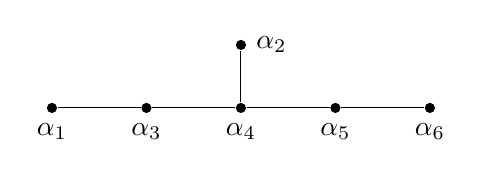
\begin{tikzpicture}[x=12mm,y=8mm,dot/.style={circle,fill,inner sep=1.3pt}]
\node[dot,label=below:{$\alpha_1$}] (a1) at (0,0) {};
\node[dot,label=below:{$\alpha_3$}] (a3) at (1,0) {};
\node[dot,label=below:{$\alpha_4$}] (a4) at (2,0) {};
\node[dot,label=below:{$\alpha_5$}] (a5) at (3,0) {};
\node[dot,label=below:{$\alpha_6$}] (a6) at (4,0) {};
\node[dot,label=right:{$\alpha_2$}] (a2) at (2,1) {};
\draw (a1)--(a3)--(a4)--(a5)--(a6) (a4)--(a2);
\end{tikzpicture}
\end{center}
After a signed permutation of the coordinates we may assume that $\phi(\alpha_4)=\Ze_1-\Ze_2$.
Two vectors of the form $\pm\Ze_i\pm\Ze_j$ have inner product $\pm1$ if and only if they share
exactly one coordinate. Thus each of $\phi(\alpha_2),\phi(\alpha_3),\phi(\alpha_5)$ is
$-\Ze_1\pm\Ze_k$ or $\Ze_2\pm\Ze_k$ with $k\notin\{1,2\}$. Two of them, say $\Zy$ and $\Zz$,
involve the same one of the coordinates $1$ and $2$, say the coordinate $1$ (the other case is
the same after the isometry $\Ze_1\leftrightarrow-\Ze_2$). Then $\Zy=-\Ze_1+\epsilon\Ze_k$ and
$\Zz=-\Ze_1+\delta\Ze_l$ with $0=\ip{\Zy}{\Zz}=1+\epsilon\delta[k=l]$, so $l=k$ and
$\Zz=-\Ze_1-\epsilon\Ze_k$. Of $\alpha_2,\alpha_3,\alpha_5$, only $\alpha_2$ is an end node (a node of valency $1$), so
one of $\Zy$, $\Zz$, say $\Zy=\phi(\beta)$, is the image of $\alpha_3$ or $\alpha_5$; let
$\gamma$ be $\alpha_1$ or $\alpha_6$ respectively, so that $\gamma$ is adjacent to $\beta$ and
orthogonal to $\alpha_4$ and to the preimage of $\Zz$. Now $\phi(\gamma)$ shares exactly one
coordinate with $\Zy$. If it involves the coordinate $1$, then $\ip{\phi(\gamma)}{\Ze_1-\Ze_2}=0$
forces $\phi(\gamma)=\pm(\Ze_1+\Ze_2)$, and then $\ip{\phi(\gamma)}{\Zz}=\mp1\ne0$. Otherwise
$\phi(\gamma)=-\epsilon\Ze_k\pm\Ze_j$ with $j\notin\{1,k\}$, and then
$\ip{\phi(\gamma)}{\Zz}=\epsilon^2=1\ne0$. Both contradict the orthogonality of $\gamma$ and
the preimage of $\Zz$.
\end{proof}

\begin{proposition}\label{prop:types}
Let $X$ be a connected graph with $\lmin(X)\ge-2$, let $r=\rk M(X)$, and let $\Phi$ be as in
Lemma~\ref{lem:rootlattice}.
\begin{enumerate}
\item $X$ is a generalized line graph if and only if $\Phi$ has type $\typ A_r$ or $\typ D_r$.
\item $X$ is exceptional if and only if $(r,\det\Lambda(X))$ is one of $(6,3)$, $(7,2)$ and
$(8,1)$, that is, if and only if $\Phi$ has type $\typ E_6$, $\typ E_7$ or $\typ E_8$.
\item $X$ is represented in $\typ E_8$ if and only if $r\le8$.
\end{enumerate}
\end{proposition}

\begin{proof}
For (1), suppose first that $\Phi$ has type $\typ A_r$ or $\typ D_r$. We will write $\Phi(R)$ for
the set of roots of the model of a root system $R$ in~\cite[\S3]{CGSS}. The isometry of~\cite[Theorem~3.5]{CGSS} maps $\Phi$ onto $\Phi(\typ A_r)$ or $\Phi(\typ D_r)$, and
$\Phi(\typ A_r)\sbs\Phi(\typ D_{r+1})$, so $X$ is represented in $\typ D_\ell$ for some $\ell$,
and it is a generalized line graph by~\cite[Theorem~4.2]{CGSS}; this is the argument of~\cite[Theorem~4.10]{CGSS}. Conversely, let $X\cong L(Y;a_1,\dots,a_m)$. By~\cite[Theorem~4.2]{CGSS}, $X$ has a
representation $(\Zy_u)$ in $\typ D_\ell\sbs\ints^\ell$. It has Gram matrix $M(X)$, so $\Lambda(X)$ is
isometric to the $\ints$-span of the $\Zy_u$, which lies in $\ints^\ell$. If $\Phi$ had type
$\typ E_k$, then $\Lambda(X)$ would contain the root lattice of $\typ E_6$ (the Dynkin diagram of
$\typ E_6$ is a subdiagram of those of $\typ E_7$ and $\typ E_8$), contradicting
Lemma~\ref{lem:E6Zm}. Thus $\Phi$ has type $\typ A_r$ or $\typ D_r$.

Part (2) follows from (1) and Lemma~\ref{lem:rootlattice}: $\typ E_r$ exists only for
$r\in\{6,7,8\}$, with determinant $9-r$, and for these $r$ the determinants $r+1$, $4$ and $9-r$
of $\typ A_r$, $\typ D_r$ and $\typ E_r$ are distinct (for $r=6$, $7$ and $8$ they are $7,4,3$;
$8,4,2$; and $9,4,1$).

For (3), a representation in $\typ E_8$ spans a space of dimension at most $8$, so $r\le8$.
Conversely, let $r\le8$. Each of $\typ A_r$, $\typ D_r$ ($r\le8$), $\typ E_6$, $\typ E_7$,
$\typ E_8$ is isometric to a subset of $\Phi(\typ E_8)$. Indeed, take the model of $\typ E_8$ in
$\re^8$ whose roots are the vectors $\pm\Ze_i\pm\Ze_j$ ($i\ne j$) and the vectors
$\tfrac12(\pm1,\dots,\pm1)$ with an even number of minus signs. The roots $\pm\Ze_i\pm\Ze_j$ form
$\typ D_8$, which contains the model $\typ D_r$ for $r\le8$, and
$\typ A_r\sbs\typ D_{r+1}\sbs\typ D_8$ for $r\le7$. For $\typ A_8$, the vectors
$\tfrac12(-1,1,1,1,1,1,1,1)$ and $\Ze_i-\Ze_{i+1}$ ($1\le i\le7$) are simple roots of an
$\typ A_8$ in the model with an odd number of minus signs, and negating a coordinate maps that
model onto the first one. Finally $\typ E_6\sbs\typ E_7\sbs\typ E_8$~\cite[\S3]{CGSS}. Composing with
the isometry of~\cite[Theorem~3.5]{CGSS}, $X$ is represented in $\typ E_8$.
\end{proof}

\section{Growing the graphs represented in \texorpdfstring{$\typ E_8$}{E8}}\label{sec:growth}

Recall that, for $n\ge1$, the level $\cS_n$ is the set of isomorphism classes of connected graphs
on $n$ vertices represented in $\typ E_8$, that is, by Proposition~\ref{prop:types}, with $M$
positive semidefinite of rank at most $8$; we will say that a graph is in $\cS_n$ when its
isomorphism class is. By~\cite[Theorem~4.3]{CGSS}, $\cS_n=\varnothing$ for $n\ge37$.

\begin{lemma}\label{lem:noncut}
Let $n\ge1$, and let $Z$ be a connected graph on $n+1$ vertices. Then $Z$ has a vertex $v$ such
that $Z-v$, the graph obtained by deleting $v$ and its edges, is connected, and $v$ has a
neighbour. If $Z$ is represented in $\typ E_8$, then so
is $Z-v$. Thus every graph in $\cS_{n+1}$ arises from a graph in $\cS_n$ by adding a vertex
adjacent to a nonempty set of vertices.
\end{lemma}

\begin{proof}
A leaf of a spanning tree is such a vertex, and it has a neighbour since $Z$ is connected and has
at least $2$ vertices. A representation of $Z$ in $\typ E_8$ restricts to one of $Z-v$.
\end{proof}

\begin{definition}\label{def:certificate}
Let $X$ be a graph on $n$ vertices and $M=M(X)$. A \textsl{certificate} for $X$ is a set $B$ of
vertices such that, in some ordering of $B$, the matrix $G=M[B,B]$ has all its leading principal
minors positive, and
\[
D\,M=M[\cdot,B]\operatorname{adj}(G)\,M[B,\cdot],\qquad D=\det G.
\]
\end{definition}

By Sylvester's criterion, the first condition says that $G$ is positive definite, so it does not
depend on the ordering. Both conditions are statements about integer matrices, which we can
check exactly.

\begin{lemma}\label{lem:certificate}
Let $X$ be a graph and $M=M(X)$. Then $X$ has a certificate if and only if $M$ is positive
semidefinite, and every certificate for $X$ has exactly $\rk M$ vertices. Further, if $M$ is
positive semidefinite, then any $\rk M$ vertices whose rows of $M$ are independent form a
certificate.
\end{lemma}

\begin{proof}
If $B$ is a certificate, then $G$ is positive definite and $M=M[\cdot,B]\,G\inv M[B,\cdot]$, so
$M$ is positive semidefinite of rank $\lvert B\rvert$, since $M[B,\cdot]$ has rank $\lvert
B\rvert$. Conversely, let $M$ be positive semidefinite of rank $r$, and let $B$ be a set of $r$
vertices whose rows of $M$ are independent. Then $M$ is the Gram matrix of vectors $\Zx_u$, and
the $\Zx_b$ ($b\in B$) are independent since their rows of $M$ are, so $G$ is positive definite
and its leading principal minors are positive. Every row $M[u,\cdot]$ is a combination
$\Zw^TM[B,\cdot]$ of the rows in $B$, and restricting to the columns in $B$ gives
$\Zw^T=M[u,B]\,G\inv$. Thus $M=M[\cdot,B]\,G\inv M[B,\cdot]$, which is the identity of
Definition~\ref{def:certificate}, since $\operatorname{adj}(G)=D\,G\inv$.
\end{proof}

For a graph $X$ and a set $N$ of vertices of $X$, we will write $X_N$ for the graph obtained from
$X$ by adding a vertex $v$ adjacent to exactly the vertices in $N$.

\begin{lemma}\label{lem:extension}
Let $X$ be a connected graph on $n$ vertices with a certificate $B$ of size $r\le8$, and let $G$,
$D$ be as in Definition~\ref{def:certificate} and $C=\operatorname{adj}(G)\,M[B,\cdot]$. For a
nonempty set $N$ of vertices of $X$, let $\Zs\in\{0,1\}^B$ be the indicator vector of
$N\cap B$. Then $X_N$ is represented in $\typ E_8$ if and only if
\begin{enumerate}
\item $\Zs^TC(\cdot,u)=D\,[u\in N]$ for every vertex $u$ of $X$, and
\item $\Zs^T\operatorname{adj}(G)\,\Zs\le2D$, with equality if $r=8$.
\end{enumerate}
\end{lemma}

\begin{proof}
$X_N$ is connected since $X$ is and $N\ne\varnothing$. Let $(\Zx_u)$ be a representation of $X$ in
$\re^r$, so that the $\Zx_b$ ($b\in B$) are a basis. Suppose first that $X_N$ is represented in
$\typ E_8$. Then $M(X_N)$ is the Gram matrix of vectors of $\re^8$, so $X_N$ has a
representation, and $M(X_N)$ has rank at most $8$. The vectors of this representation are those
of a representation of $X$, which span a space of dimension $r$, and one more vector, so they span
a space of dimension at most $r+1$. Thus $X_N$ has a representation in $\re^{r+1}\sps\re^r$, and
after an isometry of $\re^{r+1}$ we may assume that it extends $(\Zx_u)$, with the new vector
$\Zx_v$. Let $\Zp$ be the orthogonal projection of $\Zx_v$ onto $\re^r$. Then
$\ip{\Zp}{\Zx_b}=\Zs(b)$, so $\Zp=\sum_b(G\inv\Zs)(b)\Zx_b$, and, since $\Zx_v-\Zp$ is orthogonal
to every $\Zx_u$,
$\ip{\Zx_v}{\Zx_u}=\ip{\Zp}{\Zx_u}=\Zs^TG\inv M[B,u]=\Zs^TC(\cdot,u)/D$; this is condition 1,
and it holds whether or not $\Zx_v$ lies in $\re^r$. Thus the neighbours of $v$ in $X$ are
determined by $\Zs$. Further $\ip{\Zp}{\Zp}=\Zs^TG\inv\Zs\le\ip{\Zx_v}{\Zx_v}=2$, with equality
if and only if $\Zx_v\in\re^r$, which is forced when $r=8$ since the rank is at most $8$; this is
condition 2, since $\operatorname{adj}(G)=D\,G\inv$.
Conversely, if both conditions hold, let $\Zp=\sum_b(G\inv\Zs)(b)\Zx_b$, let $\Zz$ be a unit
vector orthogonal to $\re^r$ in $\re^{r+1}$, and let $\Zx_v=\Zp+\sqrt{2-\ip{\Zp}{\Zp}}\,\Zz$.
Then $\ip{\Zx_v}{\Zx_v}=2$ and, by condition 1, $\ip{\Zx_v}{\Zx_u}=[u\in N]$, so we have a
representation of $X_N$ whose span has dimension $r$ or $r+1$, and at most $8$ by condition 2. By
Proposition~\ref{prop:types}, $X_N$ is represented in $\typ E_8$.
\end{proof}

Condition 1 involves $N$, while the growth will run over the vectors $\Zs$; we will now recover
$N$ from $\Zs$. With $X$, $B$, $G$, $D$ and $C$ as in Lemma~\ref{lem:extension}, we will call a
vector $\Zs\in\{0,1\}^B$ \textsl{admissible} if $\Zs^TC(\cdot,u)\in\{0,D\}$ for every vertex $u$ of
$X$ and condition 2 holds, and we will write $N_\Zs$ for the set of vertices $u$ with
$\Zs^TC(\cdot,u)=D$.

\begin{lemma}\label{lem:admissible}
Let $X$ be a connected graph with a certificate $B$ of size $r\le8$, and let $G$, $D$ and $C$ be
as in Lemma~\ref{lem:extension}. Then the nonempty sets $N$ of vertices of $X$ with $X_N$
represented in $\typ E_8$ are exactly the sets $N_\Zs$ for the nonzero admissible vectors
$\Zs\in\{0,1\}^B$. Distinct vectors give distinct sets, and the vector $\Zs$ with $N_\Zs=N$ is the
indicator vector of $N\cap B$.
\end{lemma}

\begin{proof}
Since $\operatorname{adj}(G)\,G=DI$, we have $C(b',b)=D\,[b'=b]$ for $b,b'\in B$, so
$\Zs^TC(\cdot,b)=D\,\Zs(b)$, and $\Zs$ is the indicator vector of $N_\Zs\cap B$; in particular,
distinct vectors give distinct sets. If $\Zs$ is admissible, then conditions 1 and 2 of
Lemma~\ref{lem:extension} hold for $N_\Zs$ and $\Zs$, and $N_\Zs\ne\varnothing$ when $\Zs\ne0$;
thus $X_{N_\Zs}$ is represented in $\typ E_8$ when $\Zs$ is nonzero and admissible. Conversely, if
$X_N$ is represented in $\typ E_8$ for a nonempty set $N$, then conditions 1 and 2 hold for $N$
and the indicator vector $\Zs$ of $N\cap B$, by Lemma~\ref{lem:extension}. Then $\Zs$ is
admissible and $N=N_\Zs$, and $\Zs\ne0$, since otherwise condition 1 gives $N=\varnothing$.
\end{proof}

We will call the graphs $X_{N_\Zs}$, for the nonzero admissible vectors $\Zs$, the
\textsl{children} of $X$. By Lemma~\ref{lem:admissible}, they are the graphs $X_N$ represented in
$\typ E_8$, for the nonempty sets $N$ of vertices of $X$, so they do not depend on the choice of
the certificate $B$.

A \textsl{canonical form} assigns to each graph a graph isomorphic to it, in such a way that two
graphs have the same canonical form if and only if they are isomorphic; the computation uses the
canonical form of a canonical labelling program (see Appendix~\ref{app:computation}). The next
theorem shows that the growth misses no graph and produces only graphs of the levels.

\begin{theorem}\label{thm:growth}
Let $\cL_1=\{K_1\}$ and, for $n\ge1$, let $\cL_{n+1}$ be the set of canonical forms of the
children of the graphs $X\in\cL_n$. Then every connected graph on $n$ vertices represented in
$\typ E_8$ is isomorphic to a graph in $\cL_n$, and every graph in $\cL_n$ is connected and
represented in $\typ E_8$.
\end{theorem}

\begin{proof}
By induction on $n$; the case $n=1$ is clear, since $M(K_1)=(2)$. Each graph in $\cL_{n+1}$ is
connected and represented in $\typ E_8$, since the children of a connected graph are connected
and, by Lemma~\ref{lem:admissible}, represented in $\typ E_8$. Conversely let $Z$ be a connected
graph on $n+1$ vertices represented in $\typ E_8$. By Lemma~\ref{lem:noncut} it has a vertex $v$
with $Z-v$ connected and represented in $\typ E_8$, so by induction there are $X\in\cL_n$ and an
isomorphism $\phi\colon Z-v\to X$. Let $N=\phi(N_Z(v))$, where $N_Z(v)$ is the set of neighbours
of $v$ in $Z$; it is nonempty since $Z$ is connected. Then $X_N\cong Z$ is represented in
$\typ E_8$, so $X_N$ is a child of $X$ by Lemma~\ref{lem:admissible}, and its canonical form is a
graph of $\cL_{n+1}$ isomorphic to $Z$.
\end{proof}

Since canonical forms are equal exactly for isomorphic graphs, two graphs of $\cL_n$ are
isomorphic only if they are equal; thus the growth does not produce the same graph twice, and
$\cL_n$ consists of exactly one graph from each class of $\cS_n$. We can now prove
Theorem~\ref{thm:count}.

\begin{proof}[Proof of Theorem~\ref{thm:count}]
Let $n\ge1$. By Proposition~\ref{prop:types}, the exceptional graphs on $n$ vertices are the
graphs in $\cS_n$ with $(\rk M,\det\Lambda)\in\{(6,3),(7,2),(8,1)\}$; those with $\lmin=-2$ are
those with $\rk M<n$, and those with $\lmin>-2$ are those with $\rk M=n$. Since $\cL_n$ consists
of exactly one graph from each class of $\cS_n$, the number of exceptional graphs on $n$ vertices
with $\lmin=-2$, up to isomorphism, is the number of graphs $X\in\cL_n$ with
$(\rk M(X),\det\Lambda(X))$ one of the three pairs and $\rk M(X)<n$, and the number with
$\lmin>-2$ is the number of such graphs with $\rk M(X)=n$. The program of
Appendix~\ref{app:computation} computes the sets $\cL_1,\dots,\cL_{37}$: for each graph $X$ of
each $\cL_n$, it finds a certificate $B$, so that $\rk M(X)=\lvert B\rvert$ by
Lemma~\ref{lem:certificate}, then the nonzero admissible vectors, whose graphs $X_{N_\Zs}$ are the
children of $X$, and, when $\lvert B\rvert\ge6$, $\det\Lambda(X)$ by Lemma~\ref{lem:basisdet},
all in exact integer arithmetic. It finds $\cL_{37}=\varnothing$, as it must, since
$\cS_{37}=\varnothing$. It writes the exceptional graphs of each $\cL_n$ to the files of the
database, those with $\rk M(X)<n$ and those with $\rk M(X)=n$ to separate files
(Theorem~\ref{thm:main}), and it records the number of graphs in each file; Table~\ref{tab:counts} is made from this
record, which the verification of Appendix~\ref{app:checks} checks against the files. An
exceptional graph has $6\le\rk M\le8$ and $\rk M\le n$, so there is none on fewer than $6$
vertices, $\rk M=n$ only for $n\in\{6,7,8\}$, and $\rk M<n$ only for $n\ge7$; and there is none
on more than $36$ vertices, since $\cS_n=\varnothing$ for $n\ge37$.
\end{proof}

An exceptional graph $X$ is \textsl{maximal} if it is not an induced subgraph of a larger
exceptional graph. An exceptional graph is connected, and by Lemma~\ref{lem:certificate} and
Proposition~\ref{prop:types} its certificates have $\rk M\le8$ vertices, so admissible vectors are
defined for it.

\begin{proposition}\label{prop:maximal}
Let $X$ be an exceptional graph, and let $B$ be a certificate for $X$. Then $X$ is maximal if and
only if no nonzero vector of $\{0,1\}^B$ is admissible, that is, if and only if no graph $X_N$,
for a nonempty set $N$ of vertices of $X$, is represented in $\typ E_8$.
\end{proposition}

\begin{proof}
The two conditions are equivalent by Lemma~\ref{lem:admissible}. First, an induced subgraph of a
generalized line graph is a generalized line graph: by~\cite[Theorem~4.2]{CGSS} a graph is a
generalized line graph if and only if it is represented in $\typ D_\ell$ for some $\ell$, and a
representation in $\typ D_\ell$ restricts to one of every induced subgraph. Suppose that $X$ is
not maximal, and let $Z$ be an exceptional graph containing $X$ properly as an induced subgraph.
Since $Z$ is connected, it has a vertex $v$ outside $X$ with a neighbour in $X$, and the subgraph
of $Z$ induced on $V(X)\cup\{v\}$ is $X_N$ for the nonempty set $N$ of neighbours of $v$ in $X$.
Its matrix $M$ is a principal submatrix of $M(Z)$, so it is positive semidefinite; $X_N$ is
connected, and it is not a generalized line graph, since its induced subgraph $X$ is not. Thus
$X_N$ is exceptional, so it is represented in $\typ E_8$ by Proposition~\ref{prop:types}.
Conversely, if $X_N$ is represented in $\typ E_8$ for a nonempty set $N$, then $X_N$ is connected
and $\lmin(X_N)\ge-2$, and it is not a generalized line graph, since its induced subgraph $X$ is
not. Thus $X_N$ is an exceptional graph containing $X$ properly, and $X$ is not maximal.
\end{proof}

\section{The counts by number of vertices}\label{sec:counts}

Table~\ref{tab:counts} gives the counts for each number $n$ of vertices. As there and in the
database (Appendix~\ref{app:use}), we will write \textsl{list (A)} for the exceptional graphs with
$\lmin=-2$ and \textsl{list (B)} for those with $\lmin>-2$.

\begin{table}[htbp]
\centering
\small
\begin{tabular}{rrrrrr}
\toprule
$n$ & $\lvert\cS_n\rvert$ & (A) $\lambda_{\min}=-2$ & (B) $\lambda_{\min}>-2$ & exceptional & maximal\\
\midrule
1 & $1$ & $0$ & $0$ & $0$ & $0$\\
2 & $1$ & $0$ & $0$ & $0$ & $0$\\
3 & $2$ & $0$ & $0$ & $0$ & $0$\\
4 & $6$ & $0$ & $0$ & $0$ & $0$\\
5 & $18$ & $0$ & $0$ & $0$ & $0$\\
6 & $67$ & $0$ & $20$ & $20$ & $0$\\
7 & $291$ & $51$ & $110$ & $161$ & $0$\\
8 & $1\,410$ & $585$ & $443$ & $1\,028$ & $0$\\
9 & $6\,428$ & $5\,594$ & $0$ & $5\,594$ & $0$\\
10 & $25\,584$ & $24\,097$ & $0$ & $24\,097$ & $0$\\
11 & $87\,484$ & $85\,341$ & $0$ & $85\,341$ & $0$\\
12 & $257\,048$ & $254\,444$ & $0$ & $254\,444$ & $0$\\
13 & $649\,914$ & $647\,196$ & $0$ & $647\,196$ & $0$\\
14 & $1\,418\,205$ & $1\,415\,651$ & $0$ & $1\,415\,651$ & $0$\\
15 & $2\,677\,814$ & $2\,675\,647$ & $0$ & $2\,675\,647$ & $0$\\
16 & $4\,385\,365$ & $4\,383\,688$ & $0$ & $4\,383\,688$ & $0$\\
17 & $6\,238\,430$ & $6\,237\,257$ & $0$ & $6\,237\,257$ & $0$\\
18 & $7\,714\,028$ & $7\,713\,273$ & $0$ & $7\,713\,273$ & $0$\\
19 & $8\,288\,067$ & $8\,287\,627$ & $0$ & $8\,287\,627$ & $0$\\
20 & $7\,724\,697$ & $7\,724\,461$ & $0$ & $7\,724\,461$ & $0$\\
21 & $6\,227\,347$ & $6\,227\,227$ & $0$ & $6\,227\,227$ & $0$\\
22 & $4\,324\,420$ & $4\,324\,362$ & $0$ & $4\,324\,362$ & $1$\\
23 & $2\,572\,833$ & $2\,572\,808$ & $0$ & $2\,572\,808$ & $0$\\
24 & $1\,303\,562$ & $1\,303\,551$ & $0$ & $1\,303\,551$ & $0$\\
25 & $559\,586$ & $559\,581$ & $0$ & $559\,581$ & $0$\\
26 & $203\,365$ & $203\,363$ & $0$ & $203\,363$ & $0$\\
27 & $63\,212$ & $63\,211$ & $0$ & $63\,211$ & $0$\\
28 & $17\,245$ & $17\,244$ & $0$ & $17\,244$ & $1$\\
29 & $4\,367$ & $4\,367$ & $0$ & $4\,367$ & $432$\\
30 & $1\,041$ & $1\,041$ & $0$ & $1\,041$ & $25$\\
31 & $272$ & $272$ & $0$ & $272$ & $7$\\
32 & $75$ & $75$ & $0$ & $75$ & $3$\\
33 & $22$ & $22$ & $0$ & $22$ & $1$\\
34 & $7$ & $7$ & $0$ & $7$ & $2$\\
35 & $2$ & $2$ & $0$ & $2$ & $0$\\
36 & $1$ & $1$ & $0$ & $1$ & $1$\\
\midrule
total & $54\,752\,217$ & $54\,732\,046$ & $573$ & $54\,732\,619$ & $473$\\
\bottomrule
\end{tabular}

\caption{The numbers of graphs on $n$ vertices that are connected and represented in $\typ E_8$
(the size of the level $\cS_n$), exceptional with $\lmin=-2$ (list (A)), exceptional with
$\lmin>-2$ (list (B)), exceptional, and maximal exceptional.}\label{tab:counts}
\end{table}

As we saw after Theorem~\ref{thm:growth}, $\lvert\cS_n\rvert=\lvert\cL_n\rvert$, and the program
of Appendix~\ref{app:computation} records the number of graphs of each $\cL_n$ as it writes the
level. Thus there are exactly $54\,752\,217$ connected graphs represented in $\typ E_8$ up to
isomorphism, none of them on more than $36$ vertices~\cite[Theorem~4.3]{CGSS}. By
Proposition~\ref{prop:maximal}, an exceptional graph with a certificate $B$ is maximal if and
only if no nonzero vector of $\{0,1\}^B$ is admissible; the program records the number of
nonzero admissible vectors of every graph of the levels, and the exceptional graphs for which
this number is $0$, the maximal exceptional graphs, are $473$ graphs on $22$ to $36$ vertices.
These numbers agree with those of~\cite{CLRS02} and~\cite{Cve04}, and the numbers of list (B), of
the \textsl{minimal} exceptional graphs (those with no proper induced subgraph that is
exceptional) and of the regular exceptional graphs agree with the literature as well;
Appendix~\ref{app:checks} gives the comparisons.

\section*{Acknowledgements}

We produced the formalization (Appendix~\ref{app:lean}) and the code with language-model
agents, Anthropic Claude and OpenAI Codex. Claude also helped draft the text of this
note. We thank SURF (\url{www.surf.nl}) for the support in using the National Supercomputer
Snellius.

\appendix

\section{The program and the exactness of its tests}\label{app:computation}

\subsection*{Exactness}
The program \ml{grow.py}, in the directory \ml{exceptional/database/scripts/} of the repository,
carries out the construction of Theorem~\ref{thm:growth} and the classification of
Proposition~\ref{prop:types}. Floating point is used only to propose $B$ and
$\operatorname{adj}(G)$, and each proposal is then checked in exact arithmetic.

For each graph the program proposes a set $B$ with the pivoted Cholesky factorization of
LAPACK~\cite{LAPACK99} (\ml{dpstrf} through SciPy~\cite{VGO+20}), and then checks that $B$ is a
certificate. First, it checks that the leading principal minors of $G$ are positive, by
fraction-free (Bareiss) elimination in the integers of Python~\cite{Python}, which gives $D=\det G$
exactly, as the last of them. Next, it proposes $\operatorname{adj}(G)$: the matrix $T$ obtained
by rounding $D\,G\inv$, computed in floating point, is accepted if its entries are finite and at
most $2^{r-1}$ in absolute value and $GT=DI$ holds in 64-bit integers, and otherwise
$\operatorname{adj}(G)$ is computed exactly, by Gauss-Jordan elimination over the rationals. The
bound is the one that $\operatorname{adj}(G)$ satisfies: $G$ is positive definite with diagonal
entries $2$, so $\operatorname{adj}(G)=D\,G\inv$ is positive definite, its diagonal entries are
principal minors of $G$, at most $2^{r-1}$ by Hadamard's inequality, and its other entries are
bounded by its diagonal entries. Under the bound the product $GT$ cannot overflow, and $GT=DI$
gives $T=\operatorname{adj}(G)$, since $G$ is nonsingular. Finally, it checks the identity of
Definition~\ref{def:certificate} in 64-bit integers; with $r\le8$ for the graphs of the levels,
the entries of $\operatorname{adj}(G)$ are at most $2^7$ and those of the two sides of the
identity at most $2^{15}$ in absolute value, far below $2^{63}$.

If a check fails, the program falls back to a greedy proposal of $B$, also computed in floating
point and checked in the same way, and it stops if that fails too. The result does not depend on
which proposal is used: the children of a graph do not depend on the certificate
(Lemma~\ref{lem:admissible}), and neither do $\rk M=\lvert B\rvert$ and $\det\Lambda(X)$.

Admissibility is a set of integer identities and inequalities, tested for all $2^r-1$ nonzero
$\Zs$ at once: the program computes $\Zs^TC$ and $\Zs^T\operatorname{adj}(G)\,\Zs$ for all these
$\Zs$ in 64-bit integers. These are small as well: the entries of $C$ are at most $2^{11}$ in
absolute value, since $r\le8$, those of $\operatorname{adj}(G)$ are at most $2^7$ and those of
$M$ at most $2$, so the integers of the test are at most $2^{14}$, and $D\le2^r\le2^8$ by
Hadamard's inequality. When $r\ge6$, the program computes $\det\Lambda$ by
Lemma~\ref{lem:basisdet}, as a subgroup closure in $(\ints/D\ints)^r$, in the integers of
Python, and checks that it is one of the three values $r+1$, $4$, $9-r$ allowed by
Lemma~\ref{lem:rootlattice}; when $r\le5$ the graph is not exceptional, by
Proposition~\ref{prop:types}, and $\det\Lambda$ is not computed. The program also records, for
every graph of the levels, the number of its nonzero admissible vectors, which gives the maximal exceptional graphs
(Section~\ref{sec:counts}).

\subsection*{Canonical forms}
Canonical forms are those of \ml{labelg} of nauty 2.9.3~\cite{McKP14}, in its default mode (dense
nauty, no \ml{-S} or \ml{-t}), and the graph6 strings (Appendix~\ref{app:use}) are sorted in
byte order (\ml{LC_ALL=C sort}). The canonical form depends on
the program and its version, so a user with another canonical labelling should relabel the files
before comparing strings. Duplicates are removed with \ml{sort -u} on canonical strings, which is
correct by the definition of a canonical form. Each of the worker processes of \ml{grow.py},
which share the graphs of a level, pipes the children of its graphs through
\ml{labelg -q | sort -u} under \ml{bash -o pipefail} and checks the exit
status of the pipeline, so that a failure of \ml{labelg} stops the program.

\subsection*{Software}
We used Python 3.12~\cite{Python} with NumPy 2.5~\cite{HMvdW+20} and SciPy 1.18~\cite{VGO+20},
and nauty 2.9.3~\cite{McKP14}; for the checks, PARI 2.17.3~\cite{PARI} through
cypari2 2.2.4~\cite{cypari2}, and SageMath 10.9~\cite{Sage}.


\section{The checks of the program and of its output}\label{app:checks}

Since the computation is large, we made a few sanity checks of the program and of its output;
the scripts are in the repository, with the database. For $n\le10$, an exact test of every
connected graph on $n$ vertices from nauty's \ml{geng -c} finds exactly the graphs of $\cL_n$. A
second program rereads the files and checks, with PARI~\cite{PARI}, that every listed graph is
exceptional, in the right list and listed once. A SageMath script finds the seven exceptional
strongly regular graphs~\cite[Theorem~3.12.4]{BCN89} in list (A), and none of $34$ small
generalized line graphs in the lists.

\subsection*{Comparison with the literature}
List (B) has, on $6$, $7$ and $8$ vertices, the numbers of graphs that~\cite[\S2.3 and
Table~A2]{CRS04} and~\cite{DC79} give for the exceptional graphs with $\lmin>-2$
(Section~\ref{sec:intro}), and the numbers of maximal exceptional graphs (Section~\ref{sec:counts}) agree
with~\cite{CLRS02} and~\cite{Cve04}. Cvetkovi\'c
continues the passage of~\cite{Cve04} quoted in Section~\ref{sec:intro} with ``Minimal
exceptional graphs, all having 6 vertices, were found some 25 years ago'' (see
also~\cite{CRS04}). Every exceptional graph on $6$ vertices is minimal, since an exceptional
graph has at least $6$ vertices by Proposition~\ref{prop:types}; thus the minimal exceptional
graphs are exactly the exceptional graphs on $6$ vertices, and there are $20$ of them in list
(B), as~\cite{Cve04} states.

Cvetkovi\'c also writes that ``Most of the maximal exceptional graphs (432 of them) are 29 vertex
cones''~\cite{Cve04}. The maximal exceptional graphs are divided in~\cite[Chapter~6]{CRS04}, as
reported in~\cite[\S3]{DBvV26}, into three types: (a) those with largest valency $28$, the
largest valency possible~\cite[Theorem~4.3]{CGSS}, and exactly $29$ vertices; (b) those with
largest valency $28$ and more than $29$ vertices; and (c) those with largest valency less than
$28$. De Bruyn and van Veluw state that there are $430$ graphs of type (a), $37$ of type (b) and
$6$ of type (c); a graph of type (a) is a cone (a graph with a vertex adjacent to all the others),
since its vertex of valency $28$ is adjacent to all the others. Our counts agree exactly: $430$ of
our maximal exceptional graphs have $29$ vertices and a vertex of valency $28$, $37$ have more
than $29$ vertices and a vertex of valency $28$, and $6$ have largest valency less than $28$. Two
of the last $6$ have $29$ vertices, and both have largest valency $26$:
\begin{center}
\small
\verb!\??GWWJ@}[ThijhfxLuIzom}`vx{]AyXdYijTeUxrLNEiizKkrnS[N^}@~~{~~~~Z~~~{!\\
\verb!\@G?GGBEDkLp\R[jthtTZkY|hfyk}C[xeTYjcmUyYlNHUizS[rna[N^~B~~}N^~~N~~~{!
\end{center}
Thus exactly $430$ of the $432$ maximal exceptional graphs on $29$ vertices are cones: the
number $432$ of~\cite{Cve04} is the number of all maximal exceptional graphs on $29$ vertices.

The program \ml{count_regular.py} finds $187$ regular graphs in the lists, all in list (A), in
agreement with the $187$ regular exceptional graphs of Bussemaker, Cvetkovi\'c and
Seidel~\cite{BCS} (see~\cite[\S3.11]{BCN89} and~\cite{DBvV26}). With $k$ the valency, $163$ of
them have $n=2(k+2)$, $21$ have $n=3(k+2)/2$ and $3$ have $n=4(k+2)/3$, as they must
by~\cite[Theorem~3.12.2]{BCN89}. Hoffman's ratio bound on the independence number of a
$k$-regular graph on $n$ vertices with least eigenvalue $-2$ is $2n/(k+2)$, so these are the
classes of $163$, $21$ and $3$ regular exceptional graphs of~\cite{DBvV26}, with ratio bounds
$4$, $3$ and $8/3$.


\section{The database}\label{app:use}

The files are in the directory \ml{exceptional/database/} of the repository:
\ml{minus2/nNN.g6} holds list (A), \ml{above-minus2/nNN.g6} list (B) and \ml{maximal/nNN.g6} the
maximal exceptional graphs, on \ml{NN} vertices, where \ml{NN} is $n$ written with two digits.
Each file has one graph6 string per line, sorted in byte order (Appendix~\ref{app:computation}),
and it is compressed with gzip (with suffix \ml{.gz}) when larger than 20\,MB; the
three directories take about $770$\,MB in all. A graph6 string is the compact text format for
graphs of nauty~\cite{McKP14}; SageMath~\cite{Sage} reads one with \ml{Graph(s)}, and the tools
of nauty read the files directly, but not the gzipped ones, which have to be decompressed first,
as in \ml{zcat minus2/n22.g6.gz | countg}. The file \ml{counts.json} records, for each $n$, the
numbers of graphs in the three lists, the size of $\cS_n$ and the lattice types of its graphs,
the names of the files, and the time of the growth step and that it is complete;
Table~\ref{tab:counts} is made from it. The \ml{README.md} there repeats the definitions and
gives the commands.

\subsection*{What the files contain}
Each list stores its graphs on $n$ vertices in one file; the file of list (A) on $19$, $20$ or
$21$ vertices is stored in two parts (below), which we will take together; and an absent file
means that the list has no graphs on $n$ vertices.

\begin{theorem}\label{thm:main}
Let $n\ge1$. The strings in the file of list (A) on $n$ vertices are the graph6 strings of the
canonical forms of the exceptional graphs on $n$ vertices with $\lmin=-2$, one for each
isomorphism class, and the strings in the file of list (B) on $n$ vertices are those of the
exceptional graphs on $n$ vertices with $\lmin>-2$, one for each isomorphism class. List (B) is
empty unless $n\in\{6,7,8\}$, and both lists are empty for $n\le5$ and $n\ge37$.
\end{theorem}

\begin{proof}
As in the proof of Theorem~\ref{thm:count}, the exceptional graphs on $n$ vertices are the graphs
in $\cS_n$ with $(\rk M,\det\Lambda)\in\{(6,3),(7,2),(8,1)\}$, and $\cL_n$ consists of exactly
one graph from each class of $\cS_n$; the program computes, for each $X\in\cL_n$, $\rk M(X)$ and,
when it is at least $6$, $\det\Lambda(X)$. It writes the graph6 string of $X$, which is a
canonical form, to the file of list (A) if $X$ is exceptional with $\rk M<n$, to the file of list
(B) if $X$ is exceptional with $\rk M=n$, that is, with $M$ positive definite, and to neither
file otherwise. The bounds on $n$ are those of Theorem~\ref{thm:count}.
\end{proof}

The list of maximal graphs holds the exceptional graphs for which the recorded number of nonzero
admissible vectors is $0$. By Theorem~\ref{thm:main} and Proposition~\ref{prop:maximal}, its
strings are the graph6 strings of the canonical forms of the maximal exceptional graphs, one for
each isomorphism class.

\subsection*{The two parts of the files on 19, 20 and 21 vertices}
So that every file stays under 100\,MB, each of the files of list (A) on $19$, $20$ and $21$
vertices is split in two by number of edges, at the lower median $m_0$ of the numbers of edges:
one part holds the graphs with at most $m_0$ edges and the other those with at least $m_0+1$
edges, each in byte order, and the file names give the bounds:
\begin{center}
\small
\begin{tabular}{rrlr}
\toprule
$n$ & $m_0$ & part & graphs\\
\midrule
19 & 92 & \ml{minus2/n19.edges_le_92.g6.gz} & $4\,348\,448$\\
19 & 92 & \ml{minus2/n19.edges_ge_93.g6.gz} & $3\,939\,179$\\
20 & 103 & \ml{minus2/n20.edges_le_103.g6.gz} & $4\,047\,472$\\
20 & 103 & \ml{minus2/n20.edges_ge_104.g6.gz} & $3\,676\,989$\\
21 & 115 & \ml{minus2/n21.edges_le_115.g6.gz} & $3\,392\,738$\\
21 & 115 & \ml{minus2/n21.edges_ge_116.g6.gz} & $2\,834\,489$\\
\bottomrule
\end{tabular}
\end{center}
The script \ml{split_by_edges.py} writes the parts, with a fixed gzip header so that a rerun gives
identical bytes, and checks that they merge back to the whole list line for line. The checks of
Appendix~\ref{app:checks} read the two parts together, through the function \ml{read_list} of
\ml{e8common.py}, and \ml{verify.py} also checks that every graph in a part has its number of
edges in the range of the part.

\subsection*{Regenerating and verifying}
We will give the commands as they are run in the directory \ml{exceptional/database}; the number
$13$ in them is the number of worker processes. To regenerate everything, run
\begin{center}
\ml{scripts/run_levels.sh WORKDIR DBDIR 1 37 13}
\end{center}
with nauty and Python (NumPy, SciPy) on the path. Here \ml{WORKDIR} is a scratch directory,
\ml{DBDIR} is the directory in which the script writes the lists and \ml{counts.json}, and
\ml{1 37} asks for the growth steps from $n$ to $n+1$ vertices for $1\le n<37$. With \ml{.} as
\ml{DBDIR} the script overwrites the stored files; to compare a rerun with them, give an empty directory
instead. The script writes the levels
$\cS_n$ to \ml{WORKDIR/levels/nNN.g6} and their classification (rank, lattice determinant and
number of nonzero admissible vectors of each graph) to \ml{WORKDIR/levels/infoNN.txt}; a full run
takes about $45$ minutes on $13$ cores, and the levels take $1.7$\,GB, or $3.8$\,GB with their
classification. Then run
\ml{python scripts/split_by_edges.py DBDIR/minus2/nNN.g6.gz DBDIR/minus2} for $n=19$, $20$ and
$21$, and delete the three whole files. To verify the lists and to repeat the checks of
Appendix~\ref{app:checks}, run
\begin{center}
\begin{tabular}{l}
\ml{python scripts/verify.py . 13}\\
\ml{python scripts/check_bruteforce.py n WORKDIR/levels/nNN.g6 13}\\
\ml{sage scripts/check_named.sage . WORKDIR/levels}\\
\ml{python scripts/count_regular.py . 13 OUTFILE}
\end{tabular}
\end{center}
where \ml{verify.py} also needs cypari2, and \ml{check_bruteforce.py} is meant for small $n$.

\section{The formalization of~\texorpdfstring{\cite{CGSS}}{the paper of Cameron, Goethals, Seidel and Shult} in Lean}\label{app:lean}

\begin{table}[htbp]
\centering
\small
\begin{tabular}{@{}>{\raggedright\arraybackslash}p{40mm}>{\raggedright\arraybackslash}p{108mm}@{}}
\toprule
result & Lean declaration\\
\midrule
exceptional graph (Section~\ref{sec:intro}) & \ml{SimpleGraph.IsExceptional}\\
$\det\Lambda(X)$ (Section~\ref{sec:lattices}) & \ml{SimpleGraph.latticeDet},
\ml{SimpleGraph.IsRepresentation.latticeDet_eq_det_gram}\\
Lemma~\ref{lem:latticeroots} & \ml{SimpleGraph.IsRepresentation.latticeRoots},
\ml{SimpleGraph.IsRepresentation.isStarClosed_latticeRoots},
\ml{SimpleGraph.IsRepresentation.isIndecomposable_latticeRoots},
\ml{SimpleGraph.IsRepresentation.span_latticeRoots},
\ml{SimpleGraph.IsRepresentation.isRepresentedIn_latticeRoots}\\
Lemma~\ref{lem:rootlattice} & \ml{SimpleGraph.IsRepresentation.exists_unique_root_lattice}\\
Lemma~\ref{lem:snf} & \ml{SimpleGraph.latticeDet_eq_prod_smithNormalForm}\\
Lemma~\ref{lem:basisdet} & \ml{SimpleGraph.latticeDet_eq_div_card_basisDetGroup_sq}\\
Lemma~\ref{lem:E6Zm} & \ml{LineSystem.E}$_6$\ml{.not_exists_lattice_isometry_int},
\ml{LineSystem.E}$_6$\ml{.not_exists_integral_gram_simpleRoot}\\
Proposition~\ref{prop:types} (1) &
\ml{SimpleGraph.IsRepresentation.isGeneralizedLineGraph_iff_rootType_isClassical}\\
Proposition~\ref{prop:types} (2) & \ml{SimpleGraph.isExceptional_iff_rank_latticeDet}\\
Proposition~\ref{prop:types} (3) &
\ml{SimpleGraph.isRepresentedIn_E}$_8$\ml{_iff_posSemidef_and_rank_le}\\
Lemma~\ref{lem:noncut} & \ml{SimpleGraph.Connected.exists_noncut_isRepresentedIn_E}$_8$\\
Definition~\ref{def:certificate} & \ml{Matrix.IsGramCertificate}\\
Lemma~\ref{lem:certificate} & \ml{SimpleGraph.exists_integralGramMatrix_certificate_iff},
\ml{Matrix.IsGramCertificate.card_eq_rank},
\ml{Matrix.isGramCertificate_of_linearIndependent_rows}\\
Lemma~\ref{lem:extension} & \ml{SimpleGraph.isRepresentedIn_adjoinVertex_iff}\\
Lemma~\ref{lem:admissible} & \ml{SimpleGraph.isRepresentedIn_adjoinVertex_iff_exists_admissible},
\ml{SimpleGraph.existsUnique_admissible_of_isRepresentedIn_adjoinVertex}\\
Theorem~\ref{thm:growth} & \ml{SimpleGraph.growth_represents_levels}, for every canonical form
and every choice of certificates; \ml{SimpleGraph.CanonicalForm.ofChoice} shows that a canonical
form exists\\
Theorems~\ref{thm:count} and~\ref{thm:main}, the classification &
\ml{SimpleGraph.isExceptional_and_not_posDef_iff},
\ml{SimpleGraph.isExceptional_and_posDef_iff},
\ml{SimpleGraph.IsExceptional.card_bounds},
\ml{SimpleGraph.IsExceptional.card_mem_of_posDef},
\ml{SimpleGraph.singularExceptionalGrowth_represents},
\ml{SimpleGraph.definiteExceptionalGrowth_represents}\\
Proposition~\ref{prop:maximal}, and the list of maximal graphs &
\ml{SimpleGraph.IsExceptional.isMaximalExceptional_iff_no_admissible},
\ml{SimpleGraph.IsExceptional.isMaximalExceptional_iff_no_extension},
\ml{SimpleGraph.maximalExceptionalGrowth_represents}\\
\bottomrule
\end{tabular}
\caption{The Lean statements of the results of this note, in the directory
\ml{LineGraphs/Exceptional/}, apart from those of Lemma~\ref{lem:latticeroots}, which are in
\ml{LineGraphs/Seidel/LatticeRoots.lean}; in the names, the subscripts of $\typ E_6$ and
$\typ E_8$ are Unicode subscript digits.}\label{tab:lean}
\end{table}

We have formalized~\cite{CGSS} in the proof assistant Lean 4~\cite{dMU21}, on top of its
mathematical library Mathlib~\cite{mC20}, in the directory \ml{LineGraphs/} of the repository. A
result is in Lean when its statement and its proof are written in Lean and the proof is accepted
by the kernel of Lean, a small program that accepts a step only if it follows from the axioms of
the logic and from what was proved before. Lean checks the proofs;
whether the statements say what the paper says is left to the author. Every numbered result
of~\cite{CGSS} is in Lean, apart from Remark 2.11, which only points to a characterization proved
in another paper, and the library contains no unproved step and no added axiom.

Every definition, lemma, proposition and theorem of Sections~\ref{sec:lattices}
and~\ref{sec:growth} is in Lean (Table~\ref{tab:lean}), and so are the results of~\cite{CGSS}
that they use: \cite[Theorem~3.5]{CGSS} (\ml{LineSystem.classification}),
\cite[Theorem~4.2]{CGSS} (\ml{SimpleGraph.isRepresentedIn_Dn_iff}), \cite[Theorem~4.3]{CGSS}
(\ml{SimpleGraph.IsRepresentedIn.card_le_36}) and~\cite[Theorem~4.10]{CGSS}
(\ml{SimpleGraph.hoffman}). The library gives $\lmin(X)\ge-2$ as the positive semidefiniteness of $M(X)$ over the reals,
$\lmin(X)>-2$ as positive definiteness, and $\det\Lambda(X)$ as the Gram determinant of a
$\ints$-basis of the $\ints$-span of a representation, which it proves to depend neither on the
basis nor on the representation. Of Theorems~\ref{thm:count} and~\ref{thm:main}, the library
proves the mathematical content: that the exceptional graphs on $n$ vertices are the graphs of
the level $\cS_n$ whose pair $(\rk M,\det\Lambda)$ is $(6,3)$, $(7,2)$ or $(8,1)$; that those
with $\lmin=-2$ are those with $\rk M<n$; that the growth with this classification selects one
graph from each isomorphism class of each of the three lists; and the bounds on $n$. The
mathematical content of the counts of Section~\ref{sec:counts} is Theorem~\ref{thm:growth} and
Proposition~\ref{prop:maximal}. Not in Lean are the statement of
Theorem~\ref{thm:main} about the files, the correctness of the program of
Appendix~\ref{app:computation} and of the canonical form of \ml{labelg}, and the content of
Appendices~\ref{app:computation} to~\ref{app:use}: checking the $54\,732\,619$ strings in the
kernel is out of reach.

\FloatBarrier
\begin{thebibliography}{99}
\bibitem{LAPACK99} E.~Anderson, Z.~Bai, C.~Bischof, L.~S. Blackford, J.~Demmel,
J.~Dongarra, J.~Du~Croz, A.~Greenbaum, S.~Hammarling, A.~McKenney and D.~Sorensen,
\textsl{LAPACK Users' Guide}, third edition, SIAM, 1999, \url{https://doi.org/10.1137/1.9780898719604}.
\bibitem{BCN89} A.~E. Brouwer, A.~M. Cohen and A.~Neumaier, \textsl{Distance-Regular
Graphs}, Springer, 1989, \url{https://doi.org/10.1007/978-3-642-74341-2}.
\bibitem{BCS} F.~C. Bussemaker, D.~M. Cvetkovi\'c and J.~J. Seidel, Graphs related to
exceptional root systems, in \textsl{Combinatorics (Proc. Fifth Hungarian Colloq., Keszthely,
1976)}, Colloq. Math. Soc. J\'anos Bolyai 18, North-Holland, 1978, 185--191.
\bibitem{CGSS} P.~J. Cameron, J.-M. Goethals, J.~J. Seidel and E.~E. Shult, Line graphs,
root systems, and elliptic geometry, \textsl{J. Algebra} \textbf{43} (1976), 305--327, \url{https://doi.org/10.1016/0021-8693(76)90162-9}.
\bibitem{CS99} J.~H. Conway and N.~J.~A. Sloane, \textsl{Sphere Packings, Lattices and
Groups}, third edition, Springer, 1999, \url{https://doi.org/10.1007/978-1-4757-6568-7}.
\bibitem{Cve04} D.~Cvetkovi\'c, Notes on maximal exceptional graphs, \textsl{Univ. Beograd.
Publ. Elektrotehn. Fak. Ser. Mat.} \textbf{15} (2004), 103--107, \url{https://doi.org/10.2298/PETF0415103C}.
\bibitem{CLRS02} D.~Cvetkovi\'c, M.~Lepovi\'c, P.~Rowlinson and S.~K. Simi\'c, The
maximal exceptional graphs, \textsl{J. Combin. Theory Ser. B} \textbf{86} (2002), 347--363, \url{https://doi.org/10.1006/jctb.2002.2132}.
\bibitem{CRS04} D.~Cvetkovi\'c, P.~Rowlinson and S.~Simi\'c, \textsl{Spectral
Generalizations of Line Graphs: On Graphs with Least Eigenvalue $-2$}, London Math. Soc.
Lecture Note Ser. 314, Cambridge University Press, 2004, \url{https://doi.org/10.1017/CBO9780511751752}.
\bibitem{cypari2} \textsl{cypari2}, version 2.2.4, a Python interface to PARI/GP,
\url{https://github.com/sagemath/cypari2}.
\bibitem{DBvV26} B.~De Bruyn and T.~van Veluw, Hoffman colorability of graphs with
smallest eigenvalue at least $-2$, arXiv:2603.03859, 2026.
\bibitem{dMU21} L.~de Moura and S.~Ullrich, The Lean 4 theorem prover and programming
language, in \textsl{Automated Deduction, CADE 28}, Lecture Notes in Comput. Sci. 12699, Springer,
2021, 625--635, \url{https://doi.org/10.1007/978-3-030-79876-5_37}.
\bibitem{DC79} M.~Doob and D.~Cvetkovi\'c, On spectral characterizations and embeddings of
graphs, \textsl{Linear Algebra Appl.} \textbf{27} (1979), 17--26, \url{https://doi.org/10.1016/0024-3795(79)90028-4}.
\bibitem{HMvdW+20} C.~R. Harris, K.~J. Millman, S.~J. van der Walt et al., Array
programming with NumPy, \textsl{Nature} \textbf{585} (2020), 357--362, \url{https://doi.org/10.1038/s41586-020-2649-2}.
\bibitem{Hum72} J.~E. Humphreys, \textsl{Introduction to Lie Algebras and Representation
Theory}, Springer, 1972, \url{https://doi.org/10.1007/978-1-4612-6398-2}.
\bibitem{mC20} The mathlib Community, The Lean mathematical library, in \textsl{Proceedings
of the 9th ACM SIGPLAN International Conference on Certified Programs and Proofs (CPP 2020)},
ACM, 2020, 367--381, \url{https://doi.org/10.1145/3372885.3373824}.
\bibitem{McKP14} B.~D. McKay and A.~Piperno, Practical graph isomorphism, II,
\textsl{J. Symbolic Comput.} \textbf{60} (2014), 94--112, \url{https://doi.org/10.1016/j.jsc.2013.09.003}.
\bibitem{Mor37} L.~J. Mordell, The representation of a definite quadratic form as a sum
of two others, \textsl{Ann. of Math. (2)} \textbf{38} (1937), 751--757, \url{https://doi.org/10.2307/1968831}.
\bibitem{PARI} The PARI~Group, \textsl{PARI/GP}, version 2.17.3, Univ. Bordeaux,
\url{https://pari.math.u-bordeaux.fr/}.
\bibitem{Python} Python Software Foundation, \textsl{Python}, version 3.12.14,
\url{https://www.python.org/}.
\bibitem{Sage} The SageMath Developers, \textsl{SageMath, the Sage Mathematics Software System},
version 10.9, 2026, \url{https://www.sagemath.org/}.
\bibitem{VGO+20} P.~Virtanen, R.~Gommers, T.~E. Oliphant et al., SciPy 1.0: fundamental
algorithms for scientific computing in Python, \textsl{Nature Methods} \textbf{17} (2020),
261--272, \url{https://doi.org/10.1038/s41592-019-0686-2}.
\end{thebibliography}

\end{document}
